%--------------------------------------------------------------------------------------------------
% 
\chapter{Feature Selection Using Multi-Objective Optimization}
\label{ch:feature-selection}
%--------------------------------------------------------------------------------------------------

\epigraph{Natural selection is the preservation of favored races in the struggle for life.}{\textit{Charles Darwin}}

\begin{quote}
This chapter presents the paper titled \textit{FASTENER feature selection for inference from earth observation data} by Filip Koprivec, Klemen Kenda and Beno Šircelj published in Entropy journal \cite{koprivec:2020:fastener}.
Filip Koprivec and Klemen Kenda share the first authorship of the paper.
Klemen Kenda contributed to conceptualization and methodology, validation, writing and also to project administration and funding acquisition. 
Klemen Kenda was supervising the work of the other co-authors.
\end{quote}

Feature selection represents a crucial step in optimizing model performance.
Based on evaluation criterion, feature selection methods are divided into filter and wrapper methods.
Filter methods utilize the statistical performance of the data it trains for feature evaluation and has no relation to the used learning algorithm.
On the other hand, wrapper methods use the training accuracy of learning algorithms.
Algorithms can therefore capture more specific behaviour at the expense of computational complexity.
For wrapper algorithms, feature selection represents a search in the feature space.
The task of finding a minimal feature set that yields the best possible model results is proven to be an NP problem~\cite{hua:2009:performance}.

Wrapper algorithms employ methods are used for feature selection: complete search, heuristic search, random search \cite{jia:2022:feature}.
A complete search can find the optimal solution, however it usually represents a relatively large computational cost.
To find the optimal feature subset, the $M$-feature combinations of $N$ original features must be searched. 
So in most practical situations, the search-optimized exhaustive search cannot be achieved~\cite{jia:2022:feature}.

FASTENER algorithm belongs to the family of random search approaches.
It was originally developed to be used in land-use classification based on earth observation data, however, we have shown that the algorithm performs very well also on several other use cases, including environmental and biological datasets.
FASTENER exploits entropy-based measures, such as mutual information in the crossover phase of the iterative genetic approach. 
FASTENER outperforms other multi-objective wrapper methods  in terms of converging to a (near) optimal subset of features more quickly. 
Finally, FASTENER demonstrates superior classification accuracy when compared with the similarity and information theory-based techniques typically applied in earth observation scenarios.
FASTENER was also tested on open feature selection datasets and was compared to state-of-the-art methods. 
It achieves comparable results, however, with fewer model evaluations.
FASTENER can be used in any supervised machine learning scenario.

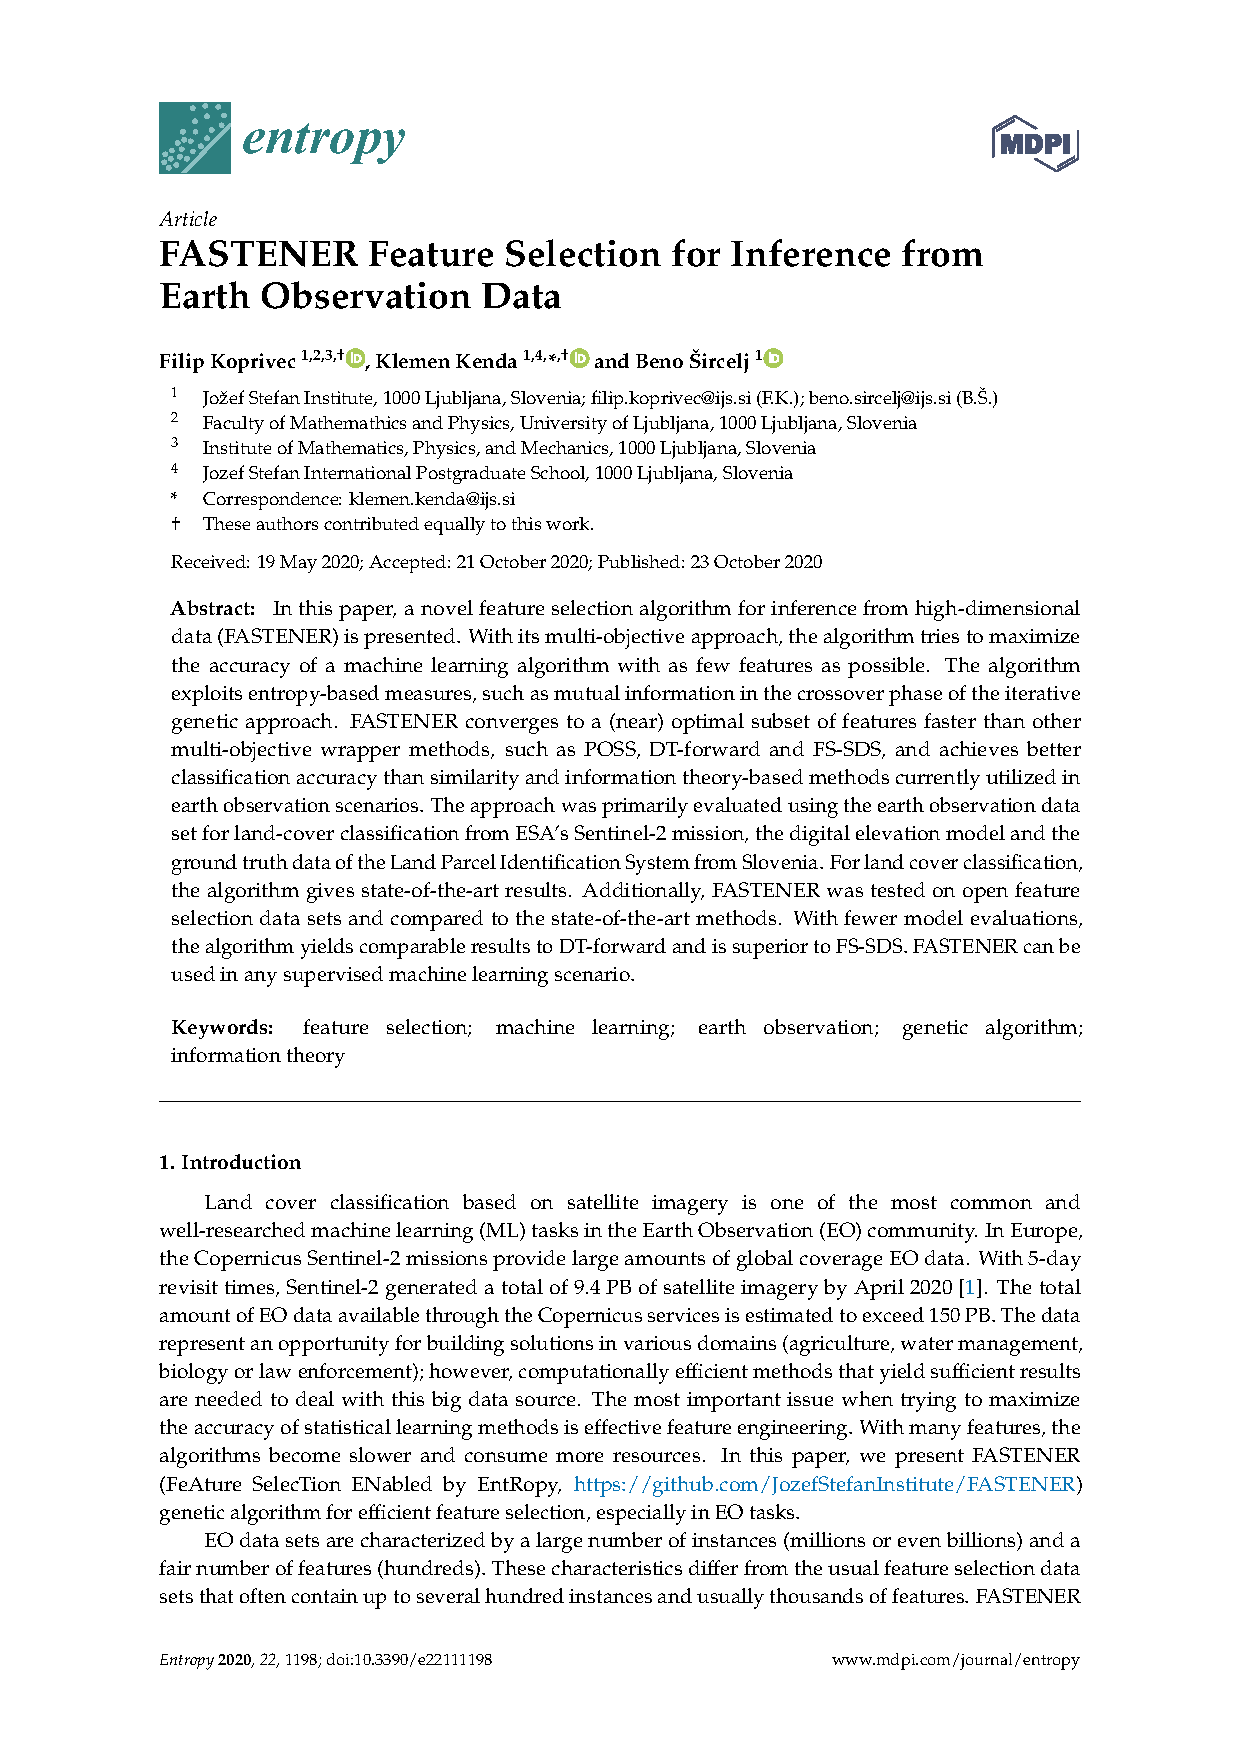
\includepdf[pages=-]{papers/fastener.pdf}
